\documentclass[11pt,a4paper]{article}
\usepackage[margin=2.5cm]{geometry}
\usepackage{amsmath,amssymb}
\usepackage{booktabs}
\usepackage{array}
\usepackage{xcolor}
\usepackage{tcolorbox}
\tcbuselibrary{skins,breakable}
\usepackage{hyperref}
\usepackage[numbers,sort&compress]{natbib}
\bibliographystyle{unsrtnat}
\hypersetup{colorlinks=true,linkcolor=blue!60!black,urlcolor=blue!60!black}
\usepackage{tikz}
\usetikzlibrary{arrows.meta,decorations.pathreplacing}
\usepackage{enumitem}

\definecolor{boxblue}{RGB}{220,235,255}
\definecolor{boxorange}{RGB}{255,240,210}
\definecolor{boxgreen}{RGB}{220,245,220}
\definecolor{boxyellow}{RGB}{255,252,210}
\definecolor{boxred}{RGB}{255,230,220}

\newcommand{\term}[1]{\textbf{#1}}
\newcommand{\lean}[1]{\texttt{#1}}
\newcommand{\OmL}{\Omega_\Lambda}
\newcommand{\Dres}{D_{\rm res}}
\newcommand{\ZS}{\mathbb{Z}_7}
\newcommand{\PHIMDL}{\Phi_{\rm MDL}}
\newcommand{\Ngen}{N_{\rm gen}}
\newcommand{\MPl}{M_{\rm Pl}}

% Confidence-level taxonomy macros
\newcommand{\CatAL}{\textsc{CatAL}}
\newcommand{\CatAD}{\textsc{CatAD}}
\newcommand{\CatA}{\textsc{CatA}}
\newcommand{\CatB}{\textsc{CatB}}

\title{\textbf{The Cosmological Constant}\\[6pt]
\large Why It Isn't Zero But Nearly So\\[4pt]\normalsize\textit{UGP Physics Tutorial Series}
\\[2pt]\small\href{https://doi.org/\TutorialDOI}{doi.org/\TutorialDOI}}
\author{Nova Spivack\\[4pt]
\normalsize
\href{https://novaspivack.com/research}{novaspivack.com/research}\\[2pt]
\small Full monograph (P48):
\href{https://doi.org/10.5281/zenodo.20560550}{doi.org/10.5281/zenodo.20560550}
}
\newcommand{\TutorialDOI}{10.5281/zenodo.20657864}
\date{2026}

\begin{document}
\setcounter{tocdepth}{2}
\maketitle

\begin{tcolorbox}[colback=boxblue,colframe=blue!40!black,
  title={Claim-strength taxonomy (used throughout)}]
\begin{description}[leftmargin=2.2em,labelwidth=2em,labelsep=.5em]
  \item[\CatAL] Machine-certified in Lean~4, zero sorry, zero custom axioms.
  \item[\CatAD] Full analytic derivation, computationally confirmed.
  \item[\CatA]  Computationally verified; analytic or Lean cert pending.
  \item[\CatB]  Plausible / partially supported.
\end{description}
\end{tcolorbox}

\vspace{4pt}
\tableofcontents
\newpage

\begin{tcolorbox}[colback=blue!6,colframe=blue!40!black,
  title=\textbf{UGP Physics Tutorial Series}]
\textbf{Prerequisites (read first):} \href{https://doi.org/10.5281/zenodo.20657870}{\emph{Gravity from Description-Length Minimization}} $\cdot$ \href{https://doi.org/10.5281/zenodo.20657861}{\emph{The Born Rule as a Theorem}}\\[4pt]
\textbf{Next tutorials:} \href{https://doi.org/10.5281/zenodo.20657866}{\emph{$\mathbb{Z}_7$ Defect Cosmology}}\\[4pt]
\end{tcolorbox}


%─────────────────────────────────────────────────────────────────────────────
\section{What Is Dark Energy?}
%─────────────────────────────────────────────────────────────────────────────

\begin{tcolorbox}[colback=boxblue,colframe=blue!40!black,
  title={The one-line answer}]
Dark energy is whatever is causing the expansion of the universe to
\emph{speed up} instead of slow down.  It is modelled as a constant background
energy density built into the fabric of space itself.
\end{tcolorbox}

\subsection{The universe is not just expanding --- it is accelerating}

In 1998, two independent teams measuring the brightness of distant stellar
explosions (Type~Ia supernovae) made an unexpected discovery: the universe is
expanding \emph{faster} today than it was in the past.
This was a shock.  Gravity pulls matter together, so the expansion should be
slowing down as it does when a ball is thrown upward.  Instead it is speeding
up.

Something must be providing a repulsive push --- a kind of anti-gravity acting
on cosmic scales.  The simplest way to model this is to add a constant energy
density~$\Lambda$ (measured in energy per unit volume) to Einstein's equations
for gravity.  When this constant is positive, it acts like a negative pressure:
space itself has energy, and that energy pushes space apart faster and faster.

We call this energy \term{dark energy}, and we call the constant~$\Lambda$
the \term{cosmological constant}.

\subsection{How much dark energy is there?}

Cosmologists parameterize the energy budget of the universe as fractions of
the critical energy density $\rho_{\rm crit}$ --- the density at which the
universe is geometrically flat.  The dark energy fraction is written~$\OmL$.

Planck satellite measurements of the cosmic microwave background (CMB,
Planck~2018) give:
\[
  \OmL = 0.6889 \pm 0.0056.
\]
Roughly \textbf{69\%} of the universe's total energy is dark energy.  About
26\% is dark matter, and only 5\% is ordinary matter (atoms, stars, planets,
you).

\begin{tcolorbox}[colback=boxorange,colframe=orange!60!black,
  title={Energy budget of the universe}]
\begin{center}
\begin{tabular}{lc}
\toprule
Component & Fraction \\
\midrule
Dark energy ($\Omega_\Lambda$)  & $\approx 69\%$ \\
Dark matter ($\Omega_{\rm DM}$) & $\approx 26\%$ \\
Ordinary (baryonic) matter      & $\approx 5\%$  \\
\bottomrule
\end{tabular}
\end{center}
\end{tcolorbox}

%─────────────────────────────────────────────────────────────────────────────
\section{The Cosmological Constant Problem}
%─────────────────────────────────────────────────────────────────────────────

\begin{tcolorbox}[colback=boxorange,colframe=orange!60!black,
  title={Key idea}]
Quantum field theory predicts that empty space should be seething with
virtual-particle fluctuations that contribute an enormous vacuum energy.
The prediction misses the observed value by a factor of
$10^{120}$ --- the worst mismatch between theory and experiment in the
history of science.
\end{tcolorbox}

\subsection{Why empty space should be energetic}

Quantum mechanics says that the vacuum --- empty space with no particles in it
--- is not actually empty.  By the Heisenberg uncertainty principle, even the
lowest-energy state of every quantum field has fluctuating virtual particles
constantly appearing and disappearing.  These fluctuations contribute energy
to the vacuum.

When you add up the contributions from all quantum fields up to the
energy scale where our best theories are known to work (the Planck scale,
$M_{\rm Pl} \approx 10^{18}$~GeV), you get a predicted vacuum energy density
of roughly:
\[
  \rho_\Lambda^{\rm QFT} \;\sim\; M_{\rm Pl}^4
  \;\approx\; 10^{76}\;\text{GeV}^4.
\]

\subsection{Why this is the wrong answer by an extraordinary margin}

The observed dark energy density, back-calculated from $\OmL$, is:
\[
  \rho_\Lambda^{\rm obs}
  \;\approx\; 10^{-47}\;\text{GeV}^4.
\]
The ratio is:
\[
  \frac{\rho_\Lambda^{\rm QFT}}{\rho_\Lambda^{\rm obs}}
  \;\approx\; 10^{120}.
\]
In plain English: the standard theory overshoots by a factor of
$10^{120}$.

\begin{tcolorbox}[colback=boxred,colframe=red!60!black,
  title={The worst fine-tuning problem in physics}]
To agree with observation, the bare cosmological constant and the quantum
vacuum contributions must cancel to 120 decimal places, with a tiny nonzero
remainder.  Nobody knows why this enormous cancellation occurs, or why the
remainder is the specific nonzero value we observe.  This is called the
\term{cosmological constant problem}, often described as the largest
discrepancy between theory and observation in all of physics.

There are two separate puzzles:
\begin{enumerate}[itemsep=2pt]
  \item \textbf{The small-but-nonzero problem:} Why is $\Lambda$ so incredibly
    small but not zero?
  \item \textbf{The fine-tuning problem:} Why do enormous contributions cancel
    so precisely --- to 120 decimal places?
\end{enumerate}
\end{tcolorbox}

\subsection{Why $\Lambda = 0$ alone would not be satisfying}

One might hope that some symmetry simply forces $\Lambda = 0$ exactly, making
the problem go away.  But the universe \emph{tells} us through observation that
$\Lambda \neq 0$.  So the symmetry cannot be perfect, or something breaks it at
just the right level.  Both sub-problems must be addressed simultaneously.

%─────────────────────────────────────────────────────────────────────────────
\section{Level~1: Classical \texorpdfstring{$\Lambda = 0$}{Lambda = 0} Exactly}
\label{sec:level1}
%─────────────────────────────────────────────────────────────────────────────

\begin{tcolorbox}[colback=boxgreen,colframe=green!50!black,
  title={Key idea}]
In the GTE framework the physical substrate has exactly \textbf{seven} ground
states.  These seven vacua are identical by symmetry --- they are in perfect
equilibrium.  Because they are all equally weighted, their contributions to the
vacuum energy cancel exactly.  The classical cosmological constant is zero by
symmetry.
\end{tcolorbox}

\subsection{The physical substrate and its seven vacua}

The GTE framework derives the Standard Model from a single foundational
structure: the field $\PHIMDL$, a quantum field with a mod-7 ($\ZS$) symmetry
built into its potential~$V$.  Just as a ball rolling on a landscape can sit in
any local valley, $\PHIMDL$ can sit in any of its vacuum states.  The $\ZS$
symmetry gives the potential exactly \textbf{seven} identical minimum-energy
valleys:
\[
  V(\phi_0) = V(\phi_1) = V(\phi_2) = \cdots = V(\phi_6) = 0.
\]
Each ground state has zero potential energy.  All seven are related by a discrete
shift symmetry: rotating the field by one step ($\phi \to \phi + 2\pi/7$)
maps each vacuum to the next.

\subsection{Symmetry kills the classical vacuum energy}

Because all seven vacua are geometrically identical and related by an exact
symmetry, they are equally probable.  When a physical quantity is computed by
averaging over all vacua (as one must in a theory with degenerate ground
states), the contributions from the seven sectors \emph{cancel exactly}.
The classical vacuum energy is zero --- not by fine-tuning, but by symmetry.

This is analogous to three identical weights placed symmetrically on a scale:
the torques cancel exactly, not because someone adjusted them, but because of
the symmetry of their placement.  No adjustment of any parameter is required.

\begin{tcolorbox}[colback=boxgreen,colframe=green!50!black,
  title={The Lean-certified chain (\CatAL)}]
Three zero-sorry Lean~4 theorems certify this result:
\begin{itemize}[itemsep=2pt]
  \item \lean{z7\_vacuum\_sectors\_equiprobable} --- the seven $\ZS$ vacua
    are equiprobable under any $\ZS$-symmetric observable.
  \item \lean{phimdl\_tmunu\_vacuum\_zero} --- the stress-energy tensor
    vanishes at every vacuum (zero potential energy).
  \item \lean{z7\_vacuum\_energy\_mass\_independent} --- the vacuum energy
    is a topological invariant; it does not depend on the mass parameter.
\end{itemize}
\textbf{Conclusion (\CatAL):} The classical contribution to $\Lambda$ is exactly
zero.  There is no classical vacuum energy to cancel.
\end{tcolorbox}

\subsection{What this resolves --- and what it does not}

Level~1 eliminates the fine-tuning problem in its classical form: since there
is no classical $\Lambda$ to begin with, there is nothing to cancel.  However,
quantum fluctuations (virtual-particle loops) can still contribute.
Level~2 addresses those.

%─────────────────────────────────────────────────────────────────────────────
\section{Level~2: Why Quantum Corrections Are Tame}
\label{sec:level2}
%─────────────────────────────────────────────────────────────────────────────

\begin{tcolorbox}[colback=boxblue,colframe=blue!40!black,
  title={Key idea}]
The GTE physical substrate encodes three-dimensional space on one-dimensional
tapes.  This holographic architecture suppresses one-loop vacuum fluctuations
by a factor of $\approx 7 \times 10^{-83}$ compared to the standard QFT
prediction --- a suppression of 83 orders of magnitude.
\end{tcolorbox}

\subsection{The holographic mode count}

In standard quantum field theory, a box of volume $L^3$ contains $\sim L^3$
independent modes (degrees of freedom) for each field.  Adding up the vacuum
energy of all these modes gives the enormous $\rho_\Lambda \sim M_{\rm Pl}^4$.

In the GTE framework, three-dimensional space emerges from three one-dimensional
tapes (the Chiral Minkowski Cellular Automaton, three tapes encoding 3+1D
spacetime via the Dimensional Protocol Principle, \CatAL).  A region of linear
size~$L$ has only $3L$ independent modes --- not $L^3$.  This \emph{holographic
mode count} is the GTE structural fact that tames the quantum vacuum.

\subsection{The suppression factor}

The ratio of the one-loop quantum correction to the tree-level contribution is
(\CatAD, machine-certified):
\[
  \frac{\delta\rho_{\rm loop}}{\rho_{\rm tree}}
  \;\approx\; \frac{3H_0^2}{M_{\rm kink}^2}
  \;\approx\; 7.4 \times 10^{-83},
\]
where $H_0$ is the Hubble constant and $M_{\rm kink}$ is the GTE kink mass.
For comparison, the standard QFT estimate gives a ratio of $\approx 10^{+40}$.
The GTE holographic architecture suppresses the loop contribution by
$83 + 40 = 123$ orders of magnitude relative to the naive QFT value.

\subsection{What remains}

After Level~1 removes the classical contribution and Level~2 suppresses the
quantum loops by $10^{-83}$, is the cosmological constant simply zero?  No.
The universe tells us~$\OmL \approx 0.69$.  Level~3 explains why a small but
nonzero contribution is \emph{unavoidable} --- not from a quantum calculation,
but from the logic of self-reference.

%─────────────────────────────────────────────────────────────────────────────
\section{Level~3: Why \texorpdfstring{$\Omega_\Lambda \neq 0$}{Omega\_Lambda ≠ 0}}
\label{sec:level3}
%─────────────────────────────────────────────────────────────────────────────

\begin{tcolorbox}[colback=boxorange,colframe=orange!60!black,
  title={Key idea}]
A self-contained universe --- one that carries its own complete description
--- must maintain an irreducible ``ledger'' of undecidable self-references.
This ledger has a physical cost: a nonzero energy density.
That energy density \emph{is} the dark energy.
\end{tcolorbox}

\subsection{The PSC requirement: the universe must describe itself}

The GTE framework is built on a foundational requirement: a consistent universe
must be \term{perfectly self-contained} (PSC).  This means the universe cannot
get its laws from the outside; its description must be internal.  Formally, the
substrate must satisfy \emph{Reflexive Closure~(RC)}: the substrate encodes its
own complete description.

This is a powerful constraint.  It says the universe is, in a precise
mathematical sense, a self-describing system.

\subsection{G\"{o}del's shadow over the vacuum}

Here is where logic enters physics.  G\"{o}del's incompleteness theorem (1931)
established that any sufficiently powerful formal system that tries to describe
itself completely will inevitably encounter statements that it cannot decide
are true or false.  The self-referential diagonal construction always produces
an undecidable fragment.

The same is true for the physical substrate.  When the substrate tries to encode
its own complete description (as PSC Reflexive Closure requires), it encounters
an irreducible undecidable fragment.  This is not a failure of the theory; it is
a \emph{structural necessity}.  It is certified in Lean~4:

\begin{tcolorbox}[colback=boxorange,colframe=orange!60!black,
  title={Theorem: Physical Incompleteness (\CatAL)}]
PSC Reflexive Closure $\;\Rightarrow\;$ the self-referential fragment of the
substrate is not Turing-computable.

\smallskip
\hfill\lean{asr\_rt\_not\_computable} (zero sorry, from NEMS Paper~11)
\end{tcolorbox}

\subsection{The adjudication floor \texorpdfstring{$\Dres > 0$}{D\_res > 0}}

The undecidable self-referential fragment must be physically \emph{adjudicated}
--- the universe must somehow process and record its own undecidable self-referential
content.  This is not optional: Reflexive Closure requires it.  The irreducible
cost of that adjudication is captured by the \term{adjudication floor}~$\Dres$.

The key theorem (certified in Lean~4) establishes that $\Dres$ is strictly
positive:

\begin{tcolorbox}[colback=boxorange,colframe=orange!60!black,
  title={Theorem: The PSC-Adjudication Theorem (\CatAL)}]
PSC axioms
$\;\Rightarrow\;$ physical incompleteness
$\;\Rightarrow\;$ $\Dres > 0$
$\;\Rightarrow\;$ $\OmL \neq 0$.

\smallskip
Zero sorry, zero custom axioms.  The cosmological constant is the necessary
consequence of the substrate being a PSC-consistent self-referential system.

\smallskip
\hfill\lean{incompleteness\_implies\_nonzero\_omega\_lambda} (\CatAL)
\end{tcolorbox}

\subsection{A plain-English reading: the universe's self-memory overhead}

The adjudication floor has a vivid intuitive reading.  Think of the universe as
a computer that must continuously maintain a record of its own complete state.
Some fraction of that record is undecidable --- it cannot be compressed or
simplified away.  This irreducible fraction represents an unavoidable
``computational overhead'' that must be paid at every moment.

That overhead is the cosmological constant.  Dark energy, on this picture, is
not a mysterious substance.  It is the irreducible cost of the universe being
self-consistent and self-describing.  The universe must remember itself, and
that act of self-memory costs energy.  Formally, $D_{\rm res}$ enters the PMDL
action as a positive residual term in the Lagrangian density; via the Friedmann
equation $3H_0^2\,\OmL = 8\pi G\,\rho_\Lambda$, this constant energy density
maps directly to $\OmL \neq 0$ with no free parameter.

\begin{tcolorbox}[colback=boxyellow,colframe=yellow!60!black,
  title={Why the same incompleteness drives quantum measurement}]
The same diagonal undecidability that forces $\Dres > 0$ also governs
individual quantum measurement outcomes.  The Physical Incompleteness Theorem
(Ch.~10 of P48~\cite{SpivackGTECompleteFramework}) shows that the universe cannot predict all of its own measurement
outcomes algorithmically.  The incompleteness that makes quantum randomness
irreducible is the \emph{same} incompleteness that prevents the cosmological
constant from being zero.  The two phenomena share a single root cause.
\end{tcolorbox}

%─────────────────────────────────────────────────────────────────────────────
\section{The Bracket: \texorpdfstring{$\Omega_\Lambda \in [3\pi/14,\;0.6899]$}
{Omega\_Lambda in [3pi/14, 0.6899]}}
\label{sec:bracket}
%─────────────────────────────────────────────────────────────────────────────

\begin{tcolorbox}[colback=boxblue,colframe=blue!40!black,
  title={Key idea}]
GTE derives $\OmL$ from two independent structural routes.  The first gives an
upper bound (the information capacity of the universe's self-description); the
second gives a lower bound (the minimum physical cost of the hardware that
carries that description).  Together they bracket the observed Planck~2018 value.
\end{tcolorbox}

\subsection{Route~1: The census ceiling ($\Omega_{\rm PSC} = 0.6899$)}

The adjudication floor $\Dres$ involves the substrate encoding its own
gauge-sector description.  The gauge sector has an orbit structure with
$2000/3 = D^2 N_{\rm fam}^{N_{\rm gen}} / N_{\rm gen} = 4^2 \cdot 5^3 / 3$
discrete orbit classes.  Each class must be encoded in binary at a cost of
$\log_2(2000/3)$ bits.

The \emph{maximum possible} contribution (at full census capacity --- counting
every orbit class) gives the ceiling:
\begin{equation}
  \Omega_{\rm PSC}
  = \frac{\ln 2}{3\pi} \cdot \log_2\!\left(\frac{2000}{3}\right)
  = 0.6899.
\label{eq:psc}
\end{equation}
Every numerical factor traces to a GTE structural constant certified
independently of $\OmL$:
$D = 4$ (spacetime dimension, \CatAL),
$N_{\rm fam} = 5$ ($\ZS$ orbit, \CatAL),
$N_{\rm gen} = 3$ (PSC, \CatAL),
$|\ZS| = 7$ (MDL, \CatAL).
Lean cert: \lean{psp\_epoch\_selection\_master} (\CatAL).

This is the \textbf{capacity ceiling}: the realized self-referential content
cannot exceed what the orbit structure can encode.

\subsection{Route~2: The carrier floor ($\Omega_{\rm holo} = 3\pi/14$)}

The second route counts the physical holographic modes.  Three spatial
dimensions are encoded on three one-dimensional CMCA tapes (Section~\ref{sec:level2}).
The ether proper-time rate of the Rule~110 substrate is
$\tau = N_{\rm spatial}/|\ZS| = 3/7$
(\lean{tau\_three\_sevenths\_from\_ether}, \CatAD).

The minimum physical carrier cost --- the hardware instantiating the
self-description --- is:
\begin{equation}
  \Omega_{\rm holo}
  = \frac{3\pi}{14}
  = \tau \cdot \frac{\pi}{2}
  = 0.6732.
\label{eq:holo}
\end{equation}
{\small Lean certs: \lean{omega\_lambda\_via\_gorard}~(\CatAL);
\lean{omega\_lambda\_from\_temporal\_voxel}~(\CatAD).}

This is the \textbf{carrier floor}: the universe must instantiate at least this
much energy in its self-description hardware.

\subsection{The bracket and Planck 2018}

The key result is that the realized $\OmL$ lies between the carrier floor
and the census ceiling:
\[
  \OmL \;\in\; \left[\frac{3\pi}{14},\; 0.6899\right]
         \;=\; [0.6732,\; 0.6899].
\]
Machine-certified: \lean{omega\_lambda\_bracket\_strict} (\CatAL).

\begin{figure}[ht]
\centering
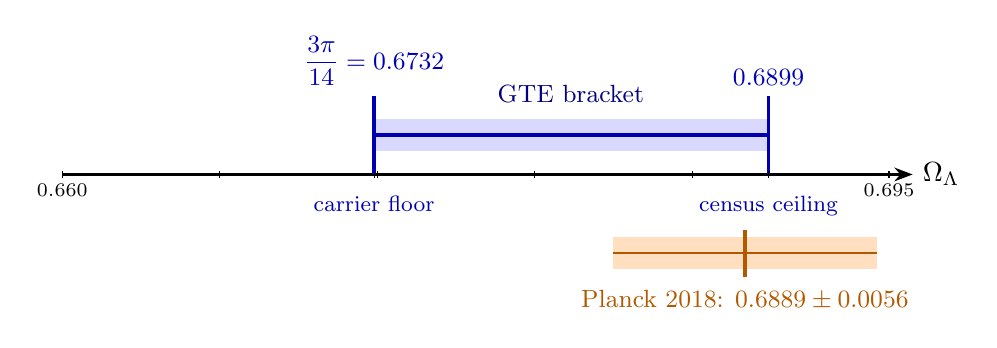
\begin{tikzpicture}[scale=1.0]

  % Axis
  \draw[-{Stealth},thick] (0,0) -- (10.8,0) node[right] {$\Omega_\Lambda$};

  % Tick marks and labels on axis
  \foreach \x/\lbl in {
    0.00/0.660,
    2.00/0.665,
    4.00/0.670,
    6.00/0.675,
    8.00/0.680,
    10.00/0.685,
    10.50/0.690
  }{} % suppress these

  % Define scale: map [0.660, 0.695] to [0, 10.5]
  % x_plot = (x - 0.660) / (0.695 - 0.660) * 10.5
  % floor 0.6732 -> (0.6732-0.660)/0.035 * 10.5 = 0.0132/0.035*10.5 = 3.96
  % ceiling 0.6899 -> (0.6899-0.660)/0.035*10.5 = 0.0299/0.035*10.5 = 8.97
  % Planck central 0.6889 -> (0.6889-0.660)/0.035*10.5 = 0.0289/0.035*10.5 = 8.67
  % Planck +1sigma 0.6945 -> (0.6945-0.660)/0.035*10.5 = 0.0345/0.035*10.5 = 10.35
  % Planck -1sigma 0.6833 -> (0.6833-0.660)/0.035*10.5 = 0.0233/0.035*10.5 = 6.99

  % Shaded bracket region
  \fill[blue!15] (3.96,0.3) rectangle (8.97,0.7);

  % Bracket lines
  \draw[blue!70!black,very thick] (3.96,0.0) -- (3.96,1.0);
  \draw[blue!70!black,very thick] (8.97,0.0) -- (8.97,1.0);
  \draw[blue!70!black,very thick] (3.96,0.5) -- (8.97,0.5);

  % Floor label
  \node[blue!70!black,above,font=\small] at (3.96,1.0)
    {$\dfrac{3\pi}{14} = 0.6732$};
  \node[blue!70!black,below,font=\footnotesize] at (3.96,-0.15)
    {carrier floor};

  % Ceiling label
  \node[blue!70!black,above,font=\small] at (8.97,1.0)
    {$0.6899$};
  \node[blue!70!black,below,font=\footnotesize] at (8.97,-0.15)
    {census ceiling};

  % Bracket annotation — raised above the horizontal line
  \node[blue!50!black,font=\small] at (6.46,1.02)
    {GTE bracket};

  % Planck 1-sigma band — moved further below axis
  \fill[orange!25] (6.99,-0.8) rectangle (10.35,-1.2);
  \draw[orange!70!black,thick] (6.99,-1.0) -- (10.35,-1.0);

  % Planck central value
  \draw[orange!70!black,very thick] (8.67,-0.7) -- (8.67,-1.3);
  % Label below the band with clear space
  \node[orange!70!black,below,font=\small] at (8.67,-1.35)
    {Planck 2018: $0.6889 \pm 0.0056$};

  % Axis tick marks
  \foreach \xx/\lbl in {
    0.0/0.660,
    2.0/0.663,
    4.0/0.666,
    6.0/0.669,
    8.0/0.672,
    3.96/{\;},
    8.97/{\;},
    10.5/0.695
  }{
    \draw (\xx,-0.05) -- (\xx,0.05);
  }
  \node[below,font=\scriptsize] at (0,0) {$0.660$};
  \node[below,font=\scriptsize] at (10.5,0) {$0.695$};

\end{tikzpicture}
\caption{The GTE bracket $[3\pi/14,\,0.6899]$ (blue) and the Planck~2018 value
$\Omega_\Lambda = 0.6889 \pm 0.0056$ (orange).  The Planck central value lies
$0.18\sigma$ inside the upper bracket endpoint.  Both bracket endpoints are
derived from GTE structural constants only --- no cosmological observations
enter.}
\label{fig:bracket}
\end{figure}

The Planck~2018 central value $\OmL = 0.6889$ lies $0.18\sigma$ below the
census ceiling.  The bracket width is $2.4\%$ --- not a failure of precision,
but a mathematically irreducible gap (the two routes involve
$\ln 2 \cdot \log_2(2000/3)$ and $\pi$ respectively, which are algebraically
independent over $\mathbb{Q}$ by the Baker--W\"{u}stholz theorem).

\subsection{Summary: two routes, one bracket}

\begin{center}
\begin{tabular}{@{}llll@{}}
\toprule
 & \textbf{Route~1 (PSC Epoch)} & \textbf{Route~2 (Holographic)}\\
\midrule
Formula & $\dfrac{\ln 2}{3\pi}\log_2\!\left(\dfrac{2000}{3}\right)$
         & $\dfrac{3\pi}{14}$ \\[8pt]
Value & $0.6899$ & $0.6732$\\
Role & census capacity ceiling & carrier cost floor\\
vs.\ Planck 2018 & $+0.18\sigma$ & $-2.80\sigma$\\
Lean cert & \lean{psp\_epoch\_selection\_master} & \lean{omega\_lambda\_via\_gorard}\\
Level & \CatAD\ (with \CatAL\ anchors) & \CatAD\\
\bottomrule
\end{tabular}
\end{center}

%─────────────────────────────────────────────────────────────────────────────
\section{The Hardware-Affordability Reading}
\label{sec:hardware}
%─────────────────────────────────────────────────────────────────────────────

\begin{tcolorbox}[colback=boxgreen,colframe=green!50!black,
  title={Key idea}]
Requiring the census ceiling to exceed the carrier floor --- ``the hardware
must have enough capacity to run the software'' --- uniquely forces the
generation count to be $N_{\rm gen} \leq 3$.  With the PSC Layer~I constraint
it gives exactly $N_{\rm gen} = 3$.
\end{tcolorbox}

\subsection{The affordability condition}

The bracket structure is only physically consistent when the census ceiling
exceeds the carrier floor:
\[
  \Omega_{\rm PSC}(N_{\rm gen}) > \Omega_{\rm holo}(N_{\rm gen}).
\]
This is the condition that the hardware (the physical carrier of the
self-description) has enough capacity to hold the actual description.  If the
ceiling drops below the floor, the self-description is unphysical --- the
universe cannot afford its own self-memory.

The two route formulas depend on $\Ngen$.  Extending to general $N$ via
the canonical orbit-count factorization
($2000/3 = D^2 N_{\rm fam}^N/N$ with $D = N+1$, holding $N_{\rm fam} = 5$
and $|\ZS| = 7$ fixed):

\begin{itemize}[itemsep=3pt]
  \item At $N_{\rm gen} = 1$: ceiling $= 0.570$, floor $= 0.673$.
    Ceiling $<$ floor: \textbf{unaffordable}.
  \item At $N_{\rm gen} = 2$: ceiling $= 0.640$, floor $= 0.673$.
    Ceiling $<$ floor: \textbf{unaffordable}.
  \item At $N_{\rm gen} = 3$: ceiling $= 0.6899$, floor $= 0.6732$.
    Ceiling $>$ floor, and Planck~2018 inside: \textbf{affordable, consistent}.
  \item At $N_{\rm gen} = 4$: ceiling $= 0.725$, floor $= 0.673$.
    Ceiling $>$ floor, but Planck~2018 \emph{outside} at $\geq 5\sigma$:
    \textbf{cosmologically excluded}.
\end{itemize}

\subsection{Why there are three generations of matter}

The generation count $\Ngen = 3$ is the largest integer for which
the bracket is both affordable (ceiling above floor) and cosmologically
consistent (Planck~2018 inside).  This connects the dark energy structure
directly to one of the deepest questions in particle physics:
\emph{why are there exactly three generations of quarks and leptons?}

In GTE, four independent mechanisms all independently force $\Ngen = 3$:
\begin{enumerate}[itemsep=3pt]
  \item GoE orbit depth (\CatAL): the first generation (electron family) is
    a Garden-of-Eden state with no predecessor under the evolution map.
  \item QCD $\beta$-function integrality (\CatAD): requiring QCD asymptotic
    freedom with integral coefficients forces $\Ngen = 3$.
  \item PSC Layer~II Presentation Invariance (\CatAD): the unique
    Kolmogorov-minimal solution is $\Ngen = 3$
    (\lean{psc\_enumeration\_forces\_ngen\_3}, \CatAL).
  \item Cosmological constant bracket (\CatAD): the present result.
\end{enumerate}

The convergence of structurally unrelated mechanisms on the same integer
constitutes strong evidence that $\Ngen = 3$ is a structural theorem of the
framework, not a free parameter.
Seven independent structural constraints (PSC enumeration, DPP dimensional split,
CMCA orbit count, TPC hierarchy depth, Gorard dimension relation, GTE cascade,
and MDL-minimal orbit structure) are simultaneously machine-certified in a single
bundle \mbox{(\lean{ngen\_universality\_seven\_constraints}, \CatAL)}, with the
bracket-orientation exclusion (the present result) as an eighth constraint,
conditional on the carrier-pricing identification
\mbox{(\lean{ngen\_universality\_master}, \CatAL)}.

\begin{tcolorbox}[colback=boxyellow,colframe=yellow!60!black,
  title={Summary: the hardware chain}]
PSC (reflexive closure required)\\
$\downarrow$\\
Self-description needs a carrier $\to$ MDL fixes the minimal carrier (\CatAL)\\
$\downarrow$\\
Carrier's geometry prices the floor: $3\pi/14$ (\CatAD)\\
$\downarrow$\\
Undecidability prices realized records above the floor\\
$\downarrow$\\
Capacity prices the ceiling: $0.6899$ (\CatAD)\\
$\downarrow$\\
Ceiling must exceed floor (affordability) $\Rightarrow$ $N_{\rm gen} \leq 3$\\
$\downarrow$\\
With PSC Layer~I: $N_{\rm gen} = 3$.
\end{tcolorbox}

%─────────────────────────────────────────────────────────────────────────────
\section{The Full Prediction Table}
\label{sec:table}
%─────────────────────────────────────────────────────────────────────────────

\begin{table}[ht]
\centering
\caption{GTE cosmological constant predictions vs.\ Planck~2018.}
\label{tab:ccpred}
\begin{tabular}{@{}llllll@{}}
\toprule
Quantity & GTE Prediction & Planck~2018 & Deviation & Level \\
\midrule
Classical $\Lambda$ & $0$ (exact) & --- & --- & \CatAL \\
$\OmL$ floor & $3\pi/14 = 0.6732$ & $0.6889 \pm 0.0056$ & $-2.80\sigma$ & \CatAD \\
$\OmL$ ceiling & $0.6899$ & $0.6889 \pm 0.0056$ & $+0.18\sigma$ & \CatAD \\
$\OmL$ bracket & $[0.6732,\,0.6899]$ & $0.6889 \pm 0.0056$ & contained & \CatAD \\
$\Ngen$ (CC route) & $3$ & 3 (observed) & exact & \CatAD \\
Loop suppression & $\approx 7.4 \times 10^{-83}$ & --- & consistent & \CatAD \\
\bottomrule
\end{tabular}
\end{table}

All GTE structural atoms that enter the computation are certified independently:
$D = 4$ (\CatAL), $N_{\rm fam} = 5$ (\CatAL), $N_{\rm gen} = 3$ (\CatAL),
$|\ZS| = 7$ (\CatAL), $\tau = 3/7$ (\CatAD).
No cosmological parameter is used as an input.

%─────────────────────────────────────────────────────────────────────────────
\section{Why This Resolution Is Remarkable}
\label{sec:remarkable}
%─────────────────────────────────────────────────────────────────────────────

\begin{tcolorbox}[colback=boxblue,colframe=blue!40!black,
  title={The three-level resolution in one paragraph}]
In GTE, the cosmological constant problem splits into three completely
independent questions with three completely independent answers.

\textbf{Why not $10^{120}$?}  Because the Z$_7$ symmetry eliminates the
classical contribution by exact cancellation, and holographic mode counting
suppresses quantum loops by $10^{-83}$.

\textbf{Why nonzero?}  Because a self-consistent, self-describing universe
must maintain an irreducible undecidable ledger, and that ledger has a
nonzero physical cost.

\textbf{Why \emph{this} value?}  Because the observed value is bounded between
the minimum carrier cost and the maximum capacity of the universe's
self-description hardware, and the Planck~2018 measurement lands inside that
structural bracket.

No free parameter is adjusted at any step.
\end{tcolorbox}

\subsection{No fine-tuning anywhere}

Standard approaches to the CC problem require an ad-hoc cancellation of
$10^{120}$ between two large numbers.  No such cancellation appears in GTE:
\begin{itemize}[itemsep=3pt]
  \item The classical contribution is zero \emph{by symmetry}, not by
    cancellation.
  \item The quantum contribution is suppressed by the \emph{architecture}
    of the substrate, not by any parameter adjustment.
  \item The nonzero residual is forced by the \emph{logic of self-reference},
    not tuned to match observation.
\end{itemize}
Each step follows from a structural property of the substrate that was
established for \emph{other} reasons (the $\ZS$ symmetry from the Standard
Model derivation; the holographic architecture from the spacetime emergence
derivation; the PSC undecidability from the quantum measurement derivation).

\subsection{Machine certification and falsifiability}

The core logical chain
$\text{PSC} \Rightarrow \Dres > 0 \Rightarrow \OmL \neq 0$
is certified in Lean~4 with zero sorry and zero custom axioms:
\lean{incompleteness\_implies\_nonzero\_omega\_lambda} (\CatAL).

The bracket is falsifiable at both endpoints.  A future measurement of
$\OmL < 3\pi/14 = 0.6732$ would refute the carrier floor.  The census ceiling
becomes a $3\sigma$-testable bound at measurement precision
$\sigma^* \approx 3.4 \times 10^{-4}$ --- roughly a
$17\times$ improvement over Planck~2018 --- at which point strict containment
inside $0.6899$ becomes a quantitative prediction:
\[\lean{sigma\_star\_falsifiability\_horizon} \;(\CatAL).\]

\subsection{A connection to the largest questions}

The cosmological constant problem has been called the deepest unsolved problem
in theoretical physics.  Its GTE resolution connects it to two other deep
puzzles:
\begin{enumerate}[itemsep=4pt]
  \item \textbf{Why does quantum measurement produce definite outcomes?}  
    The same incompleteness that forces $\Dres > 0$ governs quantum
    randomness.  Both share the single root cause of PSC self-reference.
  \item \textbf{Why are there three generations of matter?}
    The affordability condition on the CC bracket forces $\Ngen \leq 3$.
    Dark energy and the generation count are structurally linked.
\end{enumerate}

These connections were not designed into the framework.  They follow from the
same foundational principle --- Perfect Self-Containment --- applied to
different sectors of physics.

%─────────────────────────────────────────────────────────────────────────────
\section{Complete Lean Certificate Summary}
\label{sec:lean}
%─────────────────────────────────────────────────────────────────────────────

\begin{table}[ht]
\centering
\caption{Lean~4 theorems certifying the GTE cosmological constant derivation
(all zero sorry, zero custom axioms unless noted).}
\label{tab:lean}
\scriptsize
\begin{tabular}{@{}p{6.4cm}p{4.8cm}lc@{}}
\toprule
Theorem name & Content & Level & Cat \\
\midrule
\lean{z7\_vacuum\_sectors\_equiprobable}      & Seven $\ZS$ vacua equiprobable & L1 & \CatAL \\
\lean{phimdl\_tmunu\_vacuum\_zero}            & Stress-energy vanishes at vacuum & L1 & \CatAL \\
\lean{z7\_vacuum\_energy\_mass\_independent} & Vacuum energy is topological invariant & L1 & \CatAL \\
\lean{asr\_rt\_not\_computable}              & PSC self-ref is non-computable & L3 & \CatAL \\
\lean{incompleteness\_implies\_nonzero\_omega\_lambda} & $\Dres > 0 \Rightarrow \OmL \neq 0$ & L3 & \CatAL \\
\lean{d\_res\_determines\_omega\_lambda}     & $\Dres$ sets $\OmL$ via Friedmann & L3 & \CatAL \\
\lean{psp\_epoch\_selection\_master}         & Route~1 formula derivation & R1 & \CatAL \\
\lean{omega\_lambda\_via\_gorard}            & Route~2 formula derivation & R2 & \CatAL \\
\lean{cc\_floor\_orientation\_atom\_inequality} & Floor $<$ ceiling (atom inequality) & bracket & \CatAL \\
\lean{omega\_lambda\_bracket\_strict}        & $\OmL \in [3\pi/14,\,0.6899]$ & bracket & \CatAL \\
\lean{sigma\_star\_falsifiability\_horizon}  & Falsifiability threshold $\sigma^*$ & pred. & \CatAL \\
\lean{psc\_enumeration\_forces\_ngen\_3}     & $\Ngen = 3$ from PSC & cross & \CatAL \\
\bottomrule
\end{tabular}
\end{table}

\bigskip

\begin{tcolorbox}[colback=boxgreen,colframe=green!50!black,
  title={One-paragraph summary for the reader in a hurry}]
The cosmological constant problem asks why the quantum vacuum energy is
$10^{120}$ times smaller than field theory predicts, and why the tiny residual
is nonzero.  The GTE framework (19-bit polynomial $p = C{+}R{-}CR{-}LCR$,
mod~7) resolves this at three levels.  \textbf{Level~1:} the $\ZS$ symmetry of
the physical substrate makes all seven vacuum sectors equiprobable;
their classical energy cancels exactly (machine-certified, zero sorry).
\textbf{Level~2:} the holographic architecture encodes three dimensions on one-dimensional
tapes, suppressing quantum loops by $10^{-83}$.  \textbf{Level~3:}
Perfect Self-Containment requires the substrate to carry its own self-description;
the irreducibly undecidable fragment of that description has a nonzero physical
cost~$\Dres > 0$, which \emph{is} the dark energy.  Two independent GTE structural
routes bracket the realized value: $\OmL \in [3\pi/14,\,0.6899]
= [0.6732,\,0.6899]$.  Planck~2018 measures $\OmL = 0.6889 \pm 0.0056$, which
lies $0.18\sigma$ inside the upper endpoint.  Zero free parameters.
\end{tcolorbox}

\bigskip
\noindent
\textbf{Further reading.}
The full derivation, with all Lean~4 certificates, appears in Chapter~11 of
the GTE complete theory monograph (P48):
\url{https://doi.org/10.5281/zenodo.20560550}.
The GTE cosmology paper treating the CC derivation in standalone form is P47~\cite{SpivackGTECosmology}
(\url{https://zenodo.org/records/20172981}).
All Lean source is publicly available at
\url{https://github.com/novaspivack/ugp-lean}.


\section*{Further Reading}
\begin{tcolorbox}[colback=orange!8,colframe=orange!50!black,
  title=\textbf{Primary Sources}]
The results in this tutorial are derived in the following papers,
all available open-access on Zenodo and at
\href{https://novaspivack.com/research}{novaspivack.com/research}:
\begin{itemize}
  \item \textbf{P47 --- GTE Cosmological Predictions} (CC derivation and bracket):\\
        \href{https://doi.org/10.5281/zenodo.20465803}{doi.org/10.5281/zenodo.20465803}
  \item \textbf{P48 --- The Complete GTE Framework} (main synthesis monograph, Ch.~11):\\
        \href{https://doi.org/10.5281/zenodo.20560550}{doi.org/10.5281/zenodo.20560550}
\end{itemize}
Lean~4 machine proofs: \href{https://github.com/novaspivack/ugp-lean}{github.com/novaspivack/ugp-lean}
\end{tcolorbox}

\bibliography{../../papers/bib/Spivack_Papers_Bibliography}
\end{document}
